\documentclass[12pt, letterpaper, twoside]{article}
\usepackage[utf8]{inputenc}
\usepackage{titling}
\usepackage[utf8]{inputenc}
\usepackage[OT2,T1]{fontenc}
\usepackage[serbian]{babel}
\usepackage{amsmath}
\usepackage{amsmath}
\usepackage{mathtools}
\usepackage{cmsrb}
\usepackage[OT2,T1]{fontenc}
\usepackage[serbian]{babel}
\usepackage{amsmath}
\usepackage{tikz}
\usetikzlibrary{shapes,shadows,arrows}
\tikzstyle{line} = [draw, -stealth, thick]
\usepackage{graphicx}
\DeclareUnicodeCharacter{2212}{-}
\usepackage[export]{adjustbox}
\graphicspath{ {./images/} }
\makeatletter
\newcommand{\mathleft}{\@fleqntrue\@mathmargin0pt}
\newcommand{\mathcenter}{\@fleqnfalse}
\makeatother
\title{ % 
    Loss Functions and Robustness
    \\ }
\author{Emilija Mirković, Sanja Živanović}
\date{December 2022.}
\begin{document}
\maketitle
\begin{center}
\textbf{\large{1 Loss Functions}} 

\end{center}
We will now examine the loss functions from the previous chapter in more detail.\\
Let $X \in R^{p}$ be the input data vector and $Y \in R$ the output variable, with joint distribution $F(X,Y)$. In decision theory, the main motivation is to find the function $f(X)$ to predict the variable $Y$. Since there is an error in every prediction, a loss function,
\begin{center}
 $L(Y,f(X)$
\end{center} is introduced which tells us how much the actual data differs from the data obtained by the prediction. Basically, the loss function measures how good the prediction model is in terms of being able to predict the expected outcome. Consequently, it is always good when the loss function is as small as possible.\\
\hspace*{4ex}The best known and most used is the quadratic loss function, 
\begin{center}
$L(Y,f(X)) = (Y - f(X))^2$. 
\end{center}
For the quadratic loss function, the function $f(X)$ is found as follows:\[EPE(f) = E(Y-f(X))^2 = \int [y-f(X)^2] \,F(dx,dy),\]
where EPE is the root mean square error of prediction.
By switching to the conditional expectation, we get \[EPE(f) = E_XE_{Y|X}([Y-f(X)]^2|X)\]
As we want the minimum error, we need the minimum of this function, i.e. \[f(X)=argmin_cE_{Y|X}([Y-c]^2|X=x).\]
The minimum is reached for \[f(x)= E(Y|X=x).\]
For the absolute error, \(L(Y,f(X)) = |Y-f(X)|\), the minimum is not reached for the conditional expectation, but for the conditional median: \(m(Y|X)\).\\
\hspace*{4ex} Loss functions for classification represent the price paid for the inaccuracy of classification predictions (identifying which category a particular observation belongs to). Given $X \in R^d$ is the space of all possible input data, and $Y = \{−1, 1\}$ is the set of all outputs, i.e. predicted data. The goal of classification is to find the function $f(x) : X -> R$ that best predicts y for a given input. However, due to incomplete data or other factors, it is possible for the same input data to generate different output data, resulting in erroneous and inaccurate predictions. Therefore, a loss function is introduced that needs to be minimized.\\
\hspace*{4ex} Let $F$ be a statement. Then we define the indicator function: \[
    I(F)=
\begin{cases}
    1,& \text{if } F\\
    0,& \text{if }   \neg F
\end{cases}
\]
That is, the error function here is of the form \(L(Y,f(X)) = I(Y \neq f(X)) \). Both exponential $exp(-yf(x))$ and binomial $log(1+e^{-2Yf(x)})$ loss functions are often used.\\
\hspace*{4ex} It is possible, and often desirable, to choose different loss functions for different problems and data types. In practice, it happens that not all mistakes are equally important. For example, some classes may be considered more closely related than others, so misclassification between them is tolerable, while misclassification of unrelated classes is a problem. This is an example of a \textbf{\textit{cost sensitive classification}}.
\pagebreak

\begin{center}
\textbf{\large{2 Robustness}} 
\end{center}
\hspace*{4ex} A statistical method is robust if it is resistant to errors in the results that occurred in the process of inference and prediction. Different loss functions behave differently in the case of extreme data, i.e. data that are at the limits of acceptability.\\
\begin{center}
\textbf{\large{2.1 Robust Loss Functions for Regression}}
\end{center}

\hspace*{4ex} For regression problems, we have seen that squared and absolute error are most often used. The question arises as to which of these two to use for better performance. Since the solutions $E(Y|X = x)$ for the quadratic function and $m(Y|X)$ for the absolute function are the same for symmetric distributions, with such data it does not matter which error function we use. However, the quadratic function places greater emphasis on observations with large absolute residuals $|y_i − f(x_i)|$, thus it is less robust and its performance is significantly reduced compared to the absolute error function, in the case of distributions with a long tail. Also, they perform worse when there are a lot of outliers.\\
\begin{center}
\textbf{\large{2.2 Robust Loss Functions for Classification}}
\end{center}

\hspace*{4ex} We have already stated that exponential and binomial loss functions are used in the classification. For the joint population distribution these two loss functions have the same solution, however, this is not the case for final data sets. Both functions are monotonically decreasing in $yf(x)$. In a classification whose output is -1 or 1, $yf(x)$ has a similar role to residuals in regression. The classification rule $G(x) = sign[f(x)]$ implies that observations with positive $y_if(x_i) > 0$ are correctly classified, while observations with negative $y_if(x_i) < 0$ are incorrectly classified. The decision boundary is $f(x) = 0$. The goal of classification is to have more positive observations. Any loss function should "punish" \space negative observations more than "reward"\space positive ones, given that positive ones are already correctly classified. This is the case with exponential and binomial loss functions. With the loss indicator function, only negative $yf(x)$ is "punished", without "rewarding"\space correctly classified data.\\
\hspace*{4ex} The difference in "punishing"\space negative $yf(x)$ with binomial and exponential loss functions is in degree. With a binomial function, when $yf(x)$ decreases continuously, the penalty increases linearly, while with an exponential loss function, the penalty increases exponentially.\\
\hspace*{4ex}Therefore, the exponential function pays more attention to the observations with more negative $yf(x)$, while the binomial loss function is considered to take equal care of all data. Consequently, the binomial function is more resistant to extreme data. The figure below represents Loss functions for classification.
\begin{center}
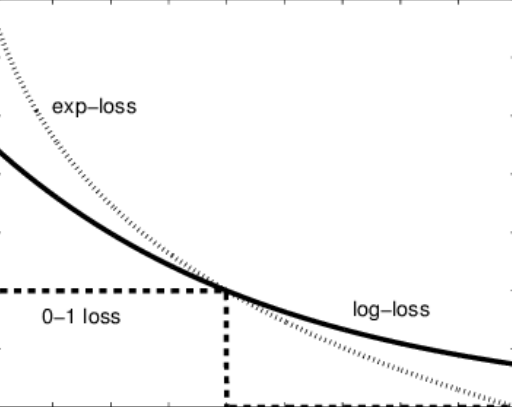
\includegraphics[width=6cm, height=5cm]{loss}
\end{center}
\hspace*{4ex}The squared error would not be a good choice for classification, primarily because it is not a monotonically decreasing function of $yf(x)$. However, there is a modification of this function, the \emph{Huber loss function}, which is more resistant to outliers and is used for both classification and regression.\\
Huber loss function for regression has the following form:
\[
    L_{\delta}(a)=
\begin{cases}
    \frac{1}{2}a^2,& \text{if } |a|\le\delta\\
    \delta(|a|-\frac{1}{2}\delta),& \text{otherwise }
\end{cases}
\]
while for the classification, it is:
\[
    L(y,f(x))=
\begin{cases}
   max(0,1-yf(x))^2,& \text{if } yf(x)\ge-1 \\
    -4yf(x),& \text{otherwise }
\end{cases}
\]
The figure below shows the relationship between the Huber, quadratic and absolute loss functions.
\begin{center}
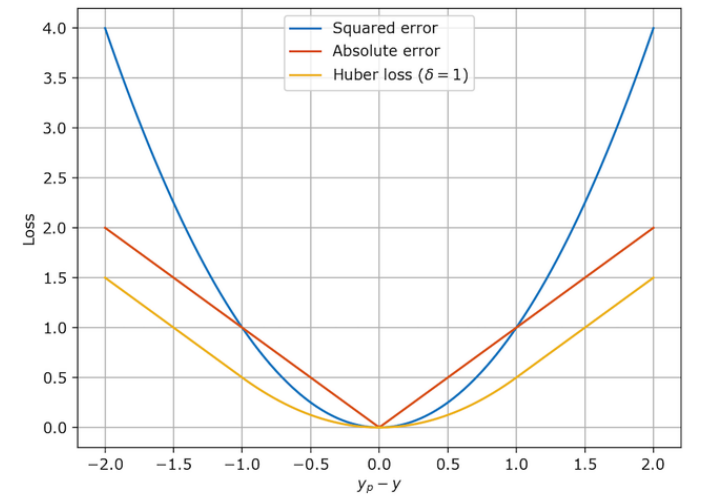
\includegraphics[width=8cm, height=6cm]{relation}
\end{center}

\begin{center}
\textbf{\large{\\3 “Off-the-Shelf” Procedures for Data Mining}\\}
\end{center}
\begin{center}
\textbf{\large{3.1 Introduction}\\}
\end{center}
\hspace*{4ex}Data mining is the process of discovering patterns in large data sets, using machine learning methods, statistics, and database systems.\\ 
\hspace*{4ex}Data mining applications can be demanding in terms of the problems they pose to learning procedures. The data is often very large, with many observations and variables. Also, the data are often unordered: they consist of a mixture of numerical and categorical variables, which usually have multiple factor levels. It happens that there are missing values or that the same data appears in more than one place. That is why, before finding a suitable model, the data is first arranged using methods of imputation, transformation, etc... Usually, only a certain portion of that data is actually meaningful for prediction, so it is very important not only to find a model that predicts well, but also to understand the data and what it shows. Therefore, models that are usually excellent for prediction, for example neural networks, are not the best choice for data mining. 
\hspace*{4ex}Due to the need for speed, easy interpretability and the generally messy nature of the data, there is a limitation in terms of using different models for prediction. An \emph{off-the-shelf} method is one that can be directly applied to the data without the need for preprocessing or adaptation.
\pagebreak
\begin{center}
\textbf{\large{\\3.2 Decision Trees}\\}
\end{center}
\hspace*{4ex}Decision trees best meet the requirements for data mining. They are relatively fast to model and provide a clear representation of the relationship between data (if they are not too large). Trees can be used on a mixture of numeric, categorical and binary data, and no imputation of missing data is required, thus freeing us from preprocessing. They are invariant to monotone data transformations, so there is no need for scaling. Another great advantage of trees is resistance to outliers.\\
\hspace*{4ex}The only drawback of trees that prevents them from being an ideal data mining tool is their imprecision. They rarely provide the precision that would be obtained using some other machine learning methods.\\
\hspace*{4ex}This problem is overcome by using boosting. Boosters drastically increase the accuracy of the model. Of course, increasing precision comes at a price: decreasing speed or interpretation. In the case of AdaBoost (Adaptive Boosting), speed, interpretation are lost, but resistance to overlapping data classes and mislabeling in the training set is also lost. The model with gradient boosting: \emph{gradient boosted mode} best maintains all the good sides of the trees, and better precision is obtained.
\begin{center}
\textbf{\large{\\4 Boosting Trees}\\}
\end{center}
\hspace*{4ex}Decision trees divide the predictor space into disjoint regions $R_j , j = 1, 2, ..., J$ which are represented by the end nodes of the tree. The constant $\gamma_j$ is assigned to each of the regions so that:
\begin{center}
$x\in R_j => f(x)=\gamma_j$
\end{center}
The tree can therefore be formally represented as:
\begin{equation*}
T(x;\Theta)=\sum_{j=1}^J\gamma_jI(x \in R_j),
\end{equation*}
with the parameter $\Theta=\{R_j,\gamma_j\}_1^J$ treated as hyperparameter. The parameters are found by minimizing the empirical risk
\begin{equation*}
\hat{\Theta}=argmin_{\Theta}\sum_{j=1}^J\sum_{x_i \in R_j}L(y_i,\gamma_i).
\end{equation*}
This is a significant combinatorial optimization problem and usually settles for approximate and sub-optimal solutions. It is useful to divide the problem into two parts:\\
\textbf{\\1. Finding $\gamma_j$ over the given $j$:} We usually use the mean value $y_i$ that falls into the region $R_j$, that is $\hat{\gamma_j}=\bar{y_i}$.\\
\textbf{\\2. Finding $R_j$:} Finding $R_j$ implies also finding $\gamma_j$. The method of top-down recursive partitioning is most often used. Additionally, it is sometimes necessary to find a smoother and more convenient approximation for $R_j$: 
\begin{equation*}
\tilde{\Theta}=argmin_{\Theta}\sum_{i=1}^N \tilde{L}(y_i,T(x_i,\Theta)).
\end{equation*}
Now we use $\hat{R_j}=\tilde{R_j}$ which gives us greater precision when finding $\gamma_j$.\\
\hspace*{4ex}The tree's \textbf{Gini index} is a measure of randomness in data sets. It aims to reduce the impurities (in terms of proper classification and partitioning) in the data, in the direction from the root nodes (at the top of the tree) to the leaf nodes (at the bottom of the tree) in the model. With the Gini index, it is possible to replace the loss obtained by wrong classification in tree growth. The boosting model is precisely the sum of such trees 
\begin{equation*}
f_M(x)=\sum_{m=1}^N T(x,\Theta_m).
\end{equation*}
induced in stages. In each step of this procedure it is necessary to calculate
\begin{equation*}
\hat{\Theta}_m=argmin_{\Theta}\sum_{i=1}^N L(y_i,f_{m-1}(x_i)+T(x_i;\Theta_m))
\end{equation*}
and the constants $\Theta_m=\{R_{jm},\gamma_{jm}\}_1^J$ of the next tree, assuming the current model $f_{m-1}(x)$.\\
\hspace*{4ex}When $R_{jm}$ is given, finding $\gamma_{jm}$ is straightforward:
\begin{equation*}
\hat{\gamma}_{jm}=argmin_{\gamma_{jm}}\sum_{x_i \in R_{jm}} L(y_i,f_{m-1}(x_i)+\gamma_{jm})
\end{equation*}
On the other hand, finding the $R_{jm}$ regions themselves is more difficult than with ordinary trees. The problem is simplified in some cases.\\
\hspace*{4ex}For the case when we have a quadratic loss function, the problem reduces to the tree that best predicts the residuals $y_i − f_{m−1}(x_i)$, where we get that $\hat{\gamma}_{jm}$ is the mean value of the residuals in the corresponding region.\\
\hspace*{4ex}In the case of exponential loss and two-class classification, the AdaBoost method is mostly used. With an absolute loss function, the solution is the median of the residuals of the corresponding region. For other criteria, there are fast iterative algorithms for finding $\hat{\gamma}_{jm}$, which give solid approximations. Simple and fast criteria for finding $\hat{\Theta}_m$ do not exist, so we decide on the approximation:
\begin{equation*}
\tilde{\Theta}=argmin_{\Theta}\sum_{i=1}^N \tilde{L}(y_i,T(x_i,\Theta)).
\end{equation*}
\end{document}





